
\chapter{X線の物理}
\section{X線の定義と発生}
X線は原子,特に核外から放出される電磁波,いわゆる光子線の一種である。その物理的性質は核内から放出される$\gamma$線と同じである。\\
\ \ X線は荷電粒子である電子を物質と衝突させることにより得られる。すなわち,電子のエネルギーが電磁放射線のエネルギーに転換した結果としてX線が発生する。\Fref{fig:Xray}に放射線医学に広く用いられているクーリッジ管方式によるX線の発生原理を示す。陰極の一部にタングステン・フィラメントを封入し,これに約10V程度の加熱電圧をかけると白熱したフィラメントから熱電子が放出される。この熱電子を高電圧で加速し,X線管球の陽極に封入された金属ターゲットに衝突させることでX線が発生する。発生するX線には「制動放射線」と「特性X線」がありX線のスペクトルは様々なエネルギーのX線光子から成る,混合エネルギースペクトルとなる。制動放射線は電子原子核近傍を通るとき,原子核の電場によって曲げられ,失った運動エネルギーとして放出される。特性X線は電子が軌道電子に衝突し,軌道電子が電離されると,できた空席にそれより高いエネルギー順位の軌道電子が落ち込むときに発生する。制動放射線はターゲットの元素には依存しないが,特性X線はターゲットによって異なる。発生したX線には透過性が低いX線も含まれるので,被写体を透過し得ないX線をあらかじめ取り除くために,射出窓には濾過版(フィルター)が設けられている。\\混合エネルギースペクトルのX線質を表す量として実効エネルギー(平均エネルギーとも呼ぶ)がある。実効エネルギーとは,連続エネルギー分布を持ったX線の半価層が単色X線の半価層\footnote{制動放射線の50$\%$透過率の厚さで定義される}と等しい時,その単色X線のエネルギーのことを実効エネルギーとして使用する。
\ \ X線のスペクトルは陰極,陽極管の加速電圧(管電圧),X線管に流れる電流(管電流)によってきまる。$P$ をX 線強度、$K$ は定数、$V $は管電圧(kV)、$I$ は管電流(mA)、$Z$ をターゲット物質の原子番号とすると
\begin{align}
P=K\times V^2\times I \times Z\label{eq:intensity}
\end{align}
ここで、管電圧設定のみ変化させたと仮定すると、\Eref{eq:intensity}からX線強度は管電圧の二乗に比例することから、臨床的によく用いられる80kVと120kVと比較すると、その差は2.25倍ということになる。管電圧を変化させるとX線強度とエネルギー両方に影響する(\Fref{fig:Xray_intensity}(左))。一方で管電流を変化させるとX線強度は変化するが、X線エネルギー(最大エネルギーや実効エネルギー)は変化しない(\Fref{fig:Xray_intensity}(右))。


\begin{figure}[H]
 \begin{center}
 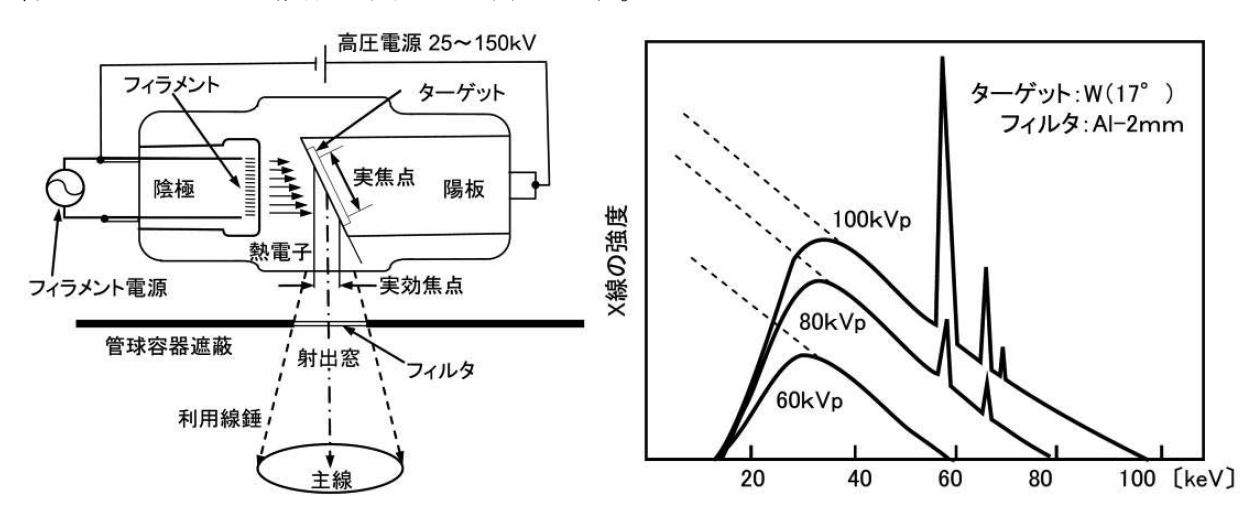
\includegraphics[bb=0.000000 0.000000 443.483339 362.370044,width=0.6\hsize]{image2/chapter2/X-ray.png} 
 \end{center}
 \caption{X線管の構造\cite{iinuma}}
 \label{fig:Xray:}
\end{figure}

\if0
\begin{figure}[H]
 \begin{center}
 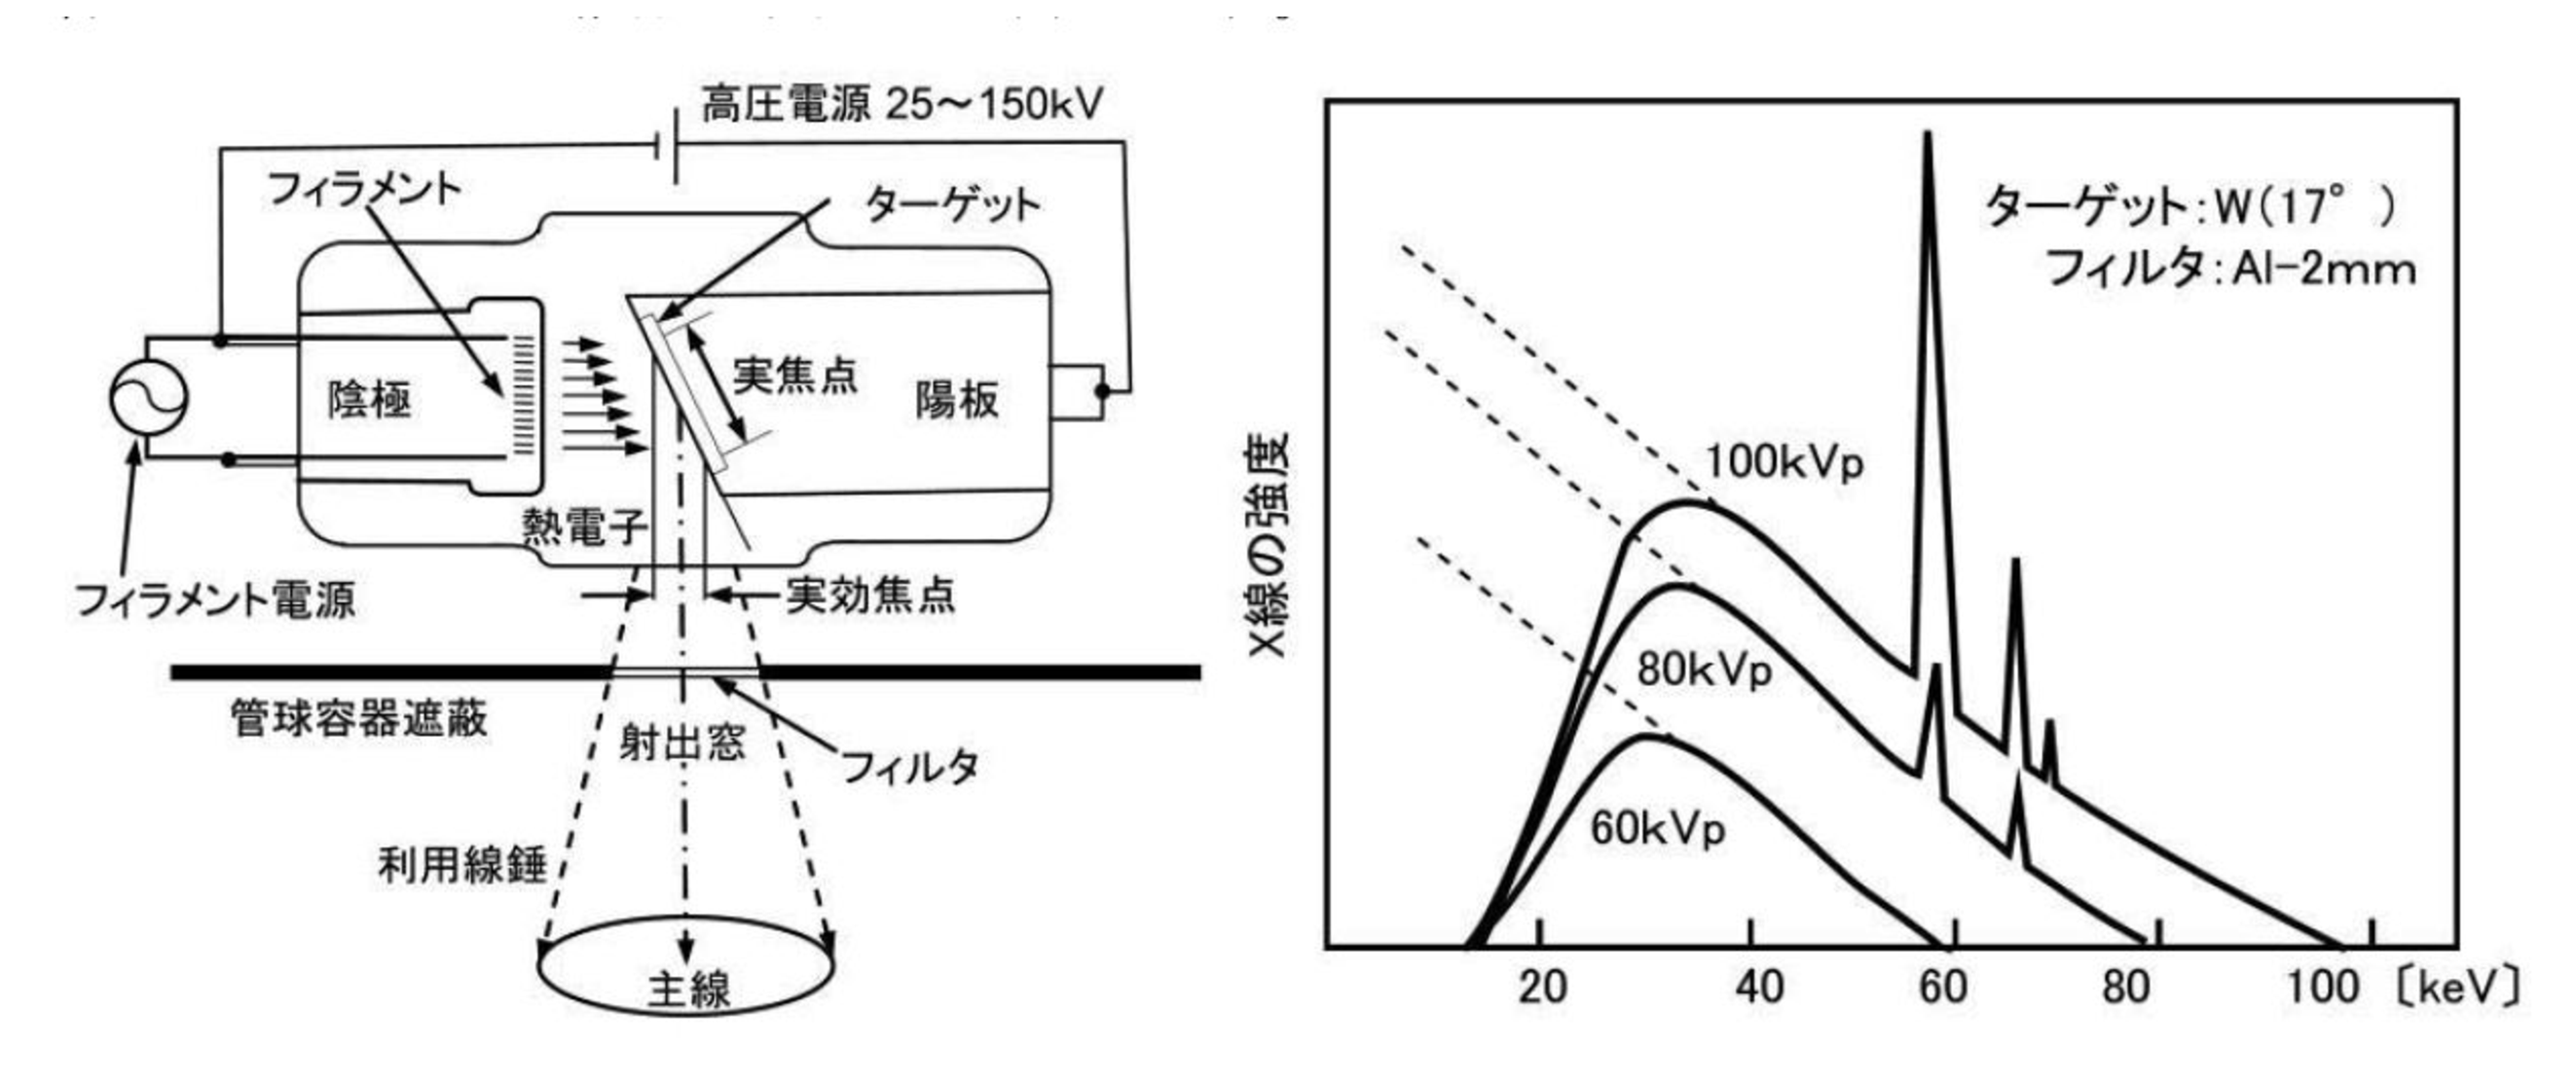
\includegraphics[width=14cm]{image/other/X-ray.eps}
 \end{center}
 \caption{X線管の構造(左)とX線スペクトル(右)\cite{iinuma}}
 \label{fig:Xray}
\end{figure}
\fi

\begin{figure}[H]
 \begin{minipage}{0.5\hsize}
  \begin{center}
   \includegraphics[bb=0.000000 0.000000 347.000000 372.000000,width=0.9\hsize]{image2/chapter2/Xray_intensity1.png} 
  \end{center}
  \vspace{0.cm}
  \caption*{管電圧を変化させた場合}
 \end{minipage}
 \begin{minipage}{0.5\hsize}
  \begin{center}
 \includegraphics[bb=0.000000 0.000000 347.000000 372.000000,width=0.9\hsize]{image2/chapter2/Xray_intensity2.png} 
  \end{center}
  \vspace{0cm}
  \caption*{管電流を変化させた場合}
 \end{minipage}
 \begin{center}
  \caption{X線のエネルギースペクトルの変化}
  \label{fig:Xray_intensity}
  \end{center}
\end{figure}



%
\if0

\subsection{$\gamma$線の定義と発生}
$\gamma$線は励起した原子核が低いエネルギー準位へ遷移する際に放出されるる電磁放射線である。本実験で用いる$\gamma$線線源の特性を\Tref{RI}に示す。

\begin{table}[H]
\begin{center}
\begin{tabular}{|l|l|l|l|l|} \hline
\multicolumn{1}{|c|}{核種} & \multicolumn{1}{c|}{半減期} & \multicolumn{1}{c|}{崩壊形式} &\parbox{12zw}{主な$\beta$線(または$\alpha$線)のエネルギーと放出の割合} & \parbox{10zw}{主な$\gamma$線のエネルギーと放出割合} \\\hline
$^{57}$Co & 271.8d & EC & 100$\%$ & 0.0144(10\%) \\
 &  &  &  & 0.122(86\%) \\
 &  &  &  & 0.136(10\%) \\
 &  &  &  & 0.0064 Fe-X \\\hline
$^{60}$Co & 5.270y & $\beta^{-}$ & 0.318(100\%) & 1.173(100\%) \\
 &  &  &  & 1.333(100\%) \\\hline
$^{109}$Cd & 463d & EC & 100\% & 0.0222\ Ag-X \\\cline{2-5}
$^{109m}$Ag & 39.6s & IT & 100\% & 0.0880(3.6\%) \\
 &  &  &  & 0.0222\ Ag-X \\\hline
$^{133}$Ba & 10.5y & EC & 100\% & 0.0810(34\%) \\
 &  &  &  & 0.276(7.2\%) \\
 &  &  &  & 0.303(18\%) \\
 &  &  &  & 0.356(62\%) \\
 &  &  &  & 0.384(8.9\%) \\
 &  &  &  & 他 \\
 &  &  &  & 0.0310\ Cs-X \\\hline
$^{241}$Am & 432.2y & $\alpha$ & 5.388(1\%) & 0.0263(2.4\%) \\
 &  &  & 5.443(13\%) & 0.0595(36\%) \\
 &  &  & 5.486(85\%) & 他 \\
 &  &  & 他 & 0.0139\ Np-LX \\\hline
\end{tabular}
\end{center}
\caption{本実験で使用する$\gamma$線線源\cite{RI}}
\label{RI}
\end{table}

\fi
%

\section{X線の物質との相互作用}
X線の物質との相互作用には光電吸収,コンプトン散乱,電子対生成がある。臨床で用いられるX線のエネルギー帯域では光電吸収,コンプトン散乱が支配的であるため、本章ではその2つの相互作用について詳細に述べる。
\subsection{光電吸収}

\begin{figure}[H]
 \begin{center}
 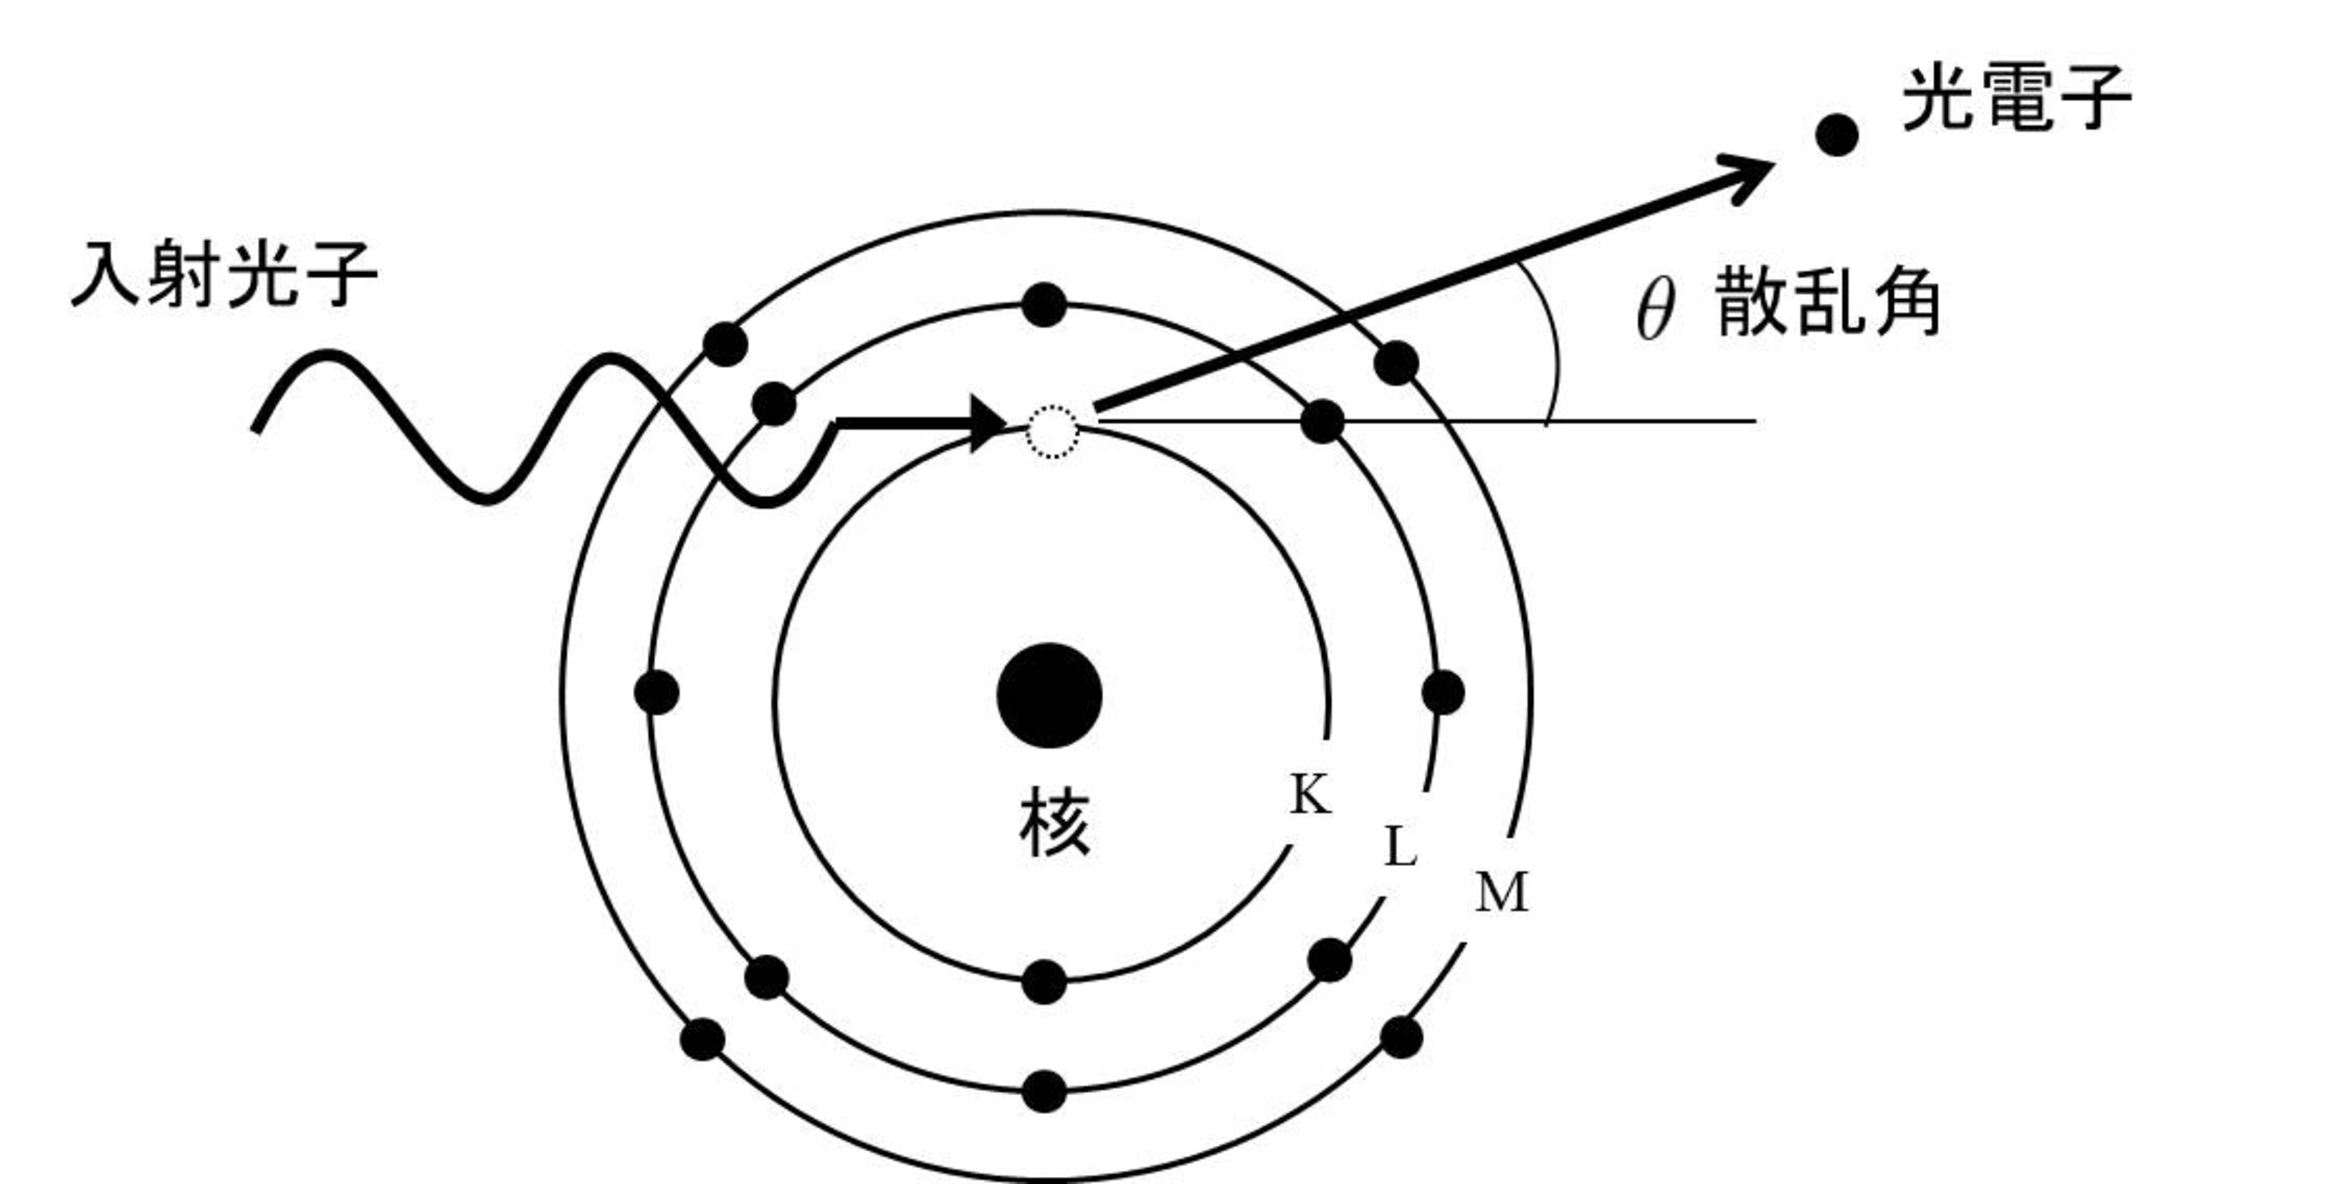
\includegraphics[width=10cm]{image/other/photo_ab.eps}
 \end{center}
 \caption{光電吸収}
 \label{fig:photo_ab}
\end{figure}

光電効果とは,物質に入射した光子が物質の軌道電子に当たり,そのエネルギーを全てその軌道電子に与え,入射した光子は消滅し軌道電子はその原子の外側へ飛び出す現象である。この原子から飛び出した軌道電子のことを光電子と呼ぶ。このとき軌道電子が原子の外に放出され,その空位の軌道を埋めるために外側の軌道電子が落ち込み,軌道電子の結合エネルギー差に相当する1個あるいはそれ以上の特性X線が放出される。いくらかの割合\footnote{放出された特性X線の光子数と光電吸収によって吸収された光子数の比を蛍光収率$\omega$といい,オージェ電子放出の割合をオージェ収率といい$(1-\omega)$で表される。K殻における蛍光収率は原子番号が高いほど高くなり,例えば$Z=75$においてはK殻において起きた光電吸収のうち93$\%$から特性X線が生じ,7$\%$からオージェ電子が生じる。逆に原子番号の低い物質の場合,蛍光収率は下がり,オージュエ収率が高くなる。}でこの結合エネルギーの差は特性X線の代わりにL殻よりゆるい結合である外側の殻から軌道電子を原子外に放出する場合がある。この電子をオージェ電子という。すなわち,軌道電子に与えられた光子のエネルギーは,最終的には光電子および付随して発生する特性X線またはオージェ電子の形でその原子の外へ放出される。\Fref{fig:photo_ab}に光電吸収の相互作用の過程を示す。光電子が受け取るエネルギー$E$は入射光子のエネルギーを$h\nu$,軌道電子の結合エネルギーを$I$とすると
\begin{align}
E=h\nu-I \label{eq:kou_ele}
\end{align}
で示される。つまり,入射光子のエネルギーは軌道電子の結合エネルギー$I$以上のエネルギーを持っている必要があり,これより光子エネルギーが小さい場合には光電吸収は起こらない。また,光電吸収は光子のエネルギーが大きすぎて,軌道電子に完全に吸収されない場合にも起こらない。1個の原子あたりの光電吸収の反応断面積$\sigma_{\rm photo}$は粗い近似式として,入射光子のエネルギー$E$,物質の原子番号を$Z$として
\begin{align}
\sigma_{\rm{photo}}\propto\frac{Z^{4-5}}{E^{3.5}} \label{eq:sigma_photo}
\end{align}
と表され,光電吸収が起きる確率は入射光子のエネルギーが低エネルギーかつ,原子番号が高い物質ほど増大する。逆に,入射光子のエネルギーが高いほど激減するため,光電吸収は高エネルギー領域では無視できる程小さくなる。しかし,鉛のように原子番号が高い元素では無視できなくなる。\\
\ \ また,光電吸収はK殻において最も起こりやすく,約80$\%$の光電吸収ががK殻で起きることが実験的に確かめられているが\footnote{K殻の軌道電子の束縛エネルギーが最も大きため,光電吸収はK殻において最も起きにくいように思われるがそれは誤りである。L殻やM殻などでは束縛エネルギーが小さいので,\Eref{eq:kou_ele}より原子から飛び出す光電子の速度が速くなるため,運動量も大きくなる。しかし,入射光子の運動量は極めて小さいため,入射光子と光電子の2体だけでは運動量保存則を満たことができず,第3体として原子核自体が反跳運動量を受け取る必要がある。したがって光電子の運動量が大きくなる,つまり束縛エネルギーが小さいほど運動量保存則を満たすことが困難となるため,束縛エネルギーの最も大きいK殻において光電吸収は最も起こりやすくなる。},L殻,M殻においても起きる。そのため入射光子のエネルギーがK殻,L殻,M殻結合エネルギーに等しくなるたびに急激に増大し不連続になる。この不連続部分を吸収端と呼ぶ。その結果,光電吸収断面積$\sigma_{\rm photo}$はジグザグを繰り返しながらエネルギーの増加とともに減少していく。

\subsection{コンプトン散乱}
入射光子のエネルギーが軌道電子の束縛エネルギーを無視できるほどになるとコンプトン散乱が起きるようになる。コンプトン散乱とは,入射光子が原子の軌道電子と衝突して,電子にエネルギーの一部を与えて弾き飛ばし,同時に入射光子自身はその分だけエネルギーを失って,波長が長くなり別の方向へ散乱される現象である(\Fref{fig:comp_geo})。弾き飛ばされた電子を反跳電子,散乱された光子を散乱光子と呼ぶ。

\begin{figure}[H]
 \begin{center}
 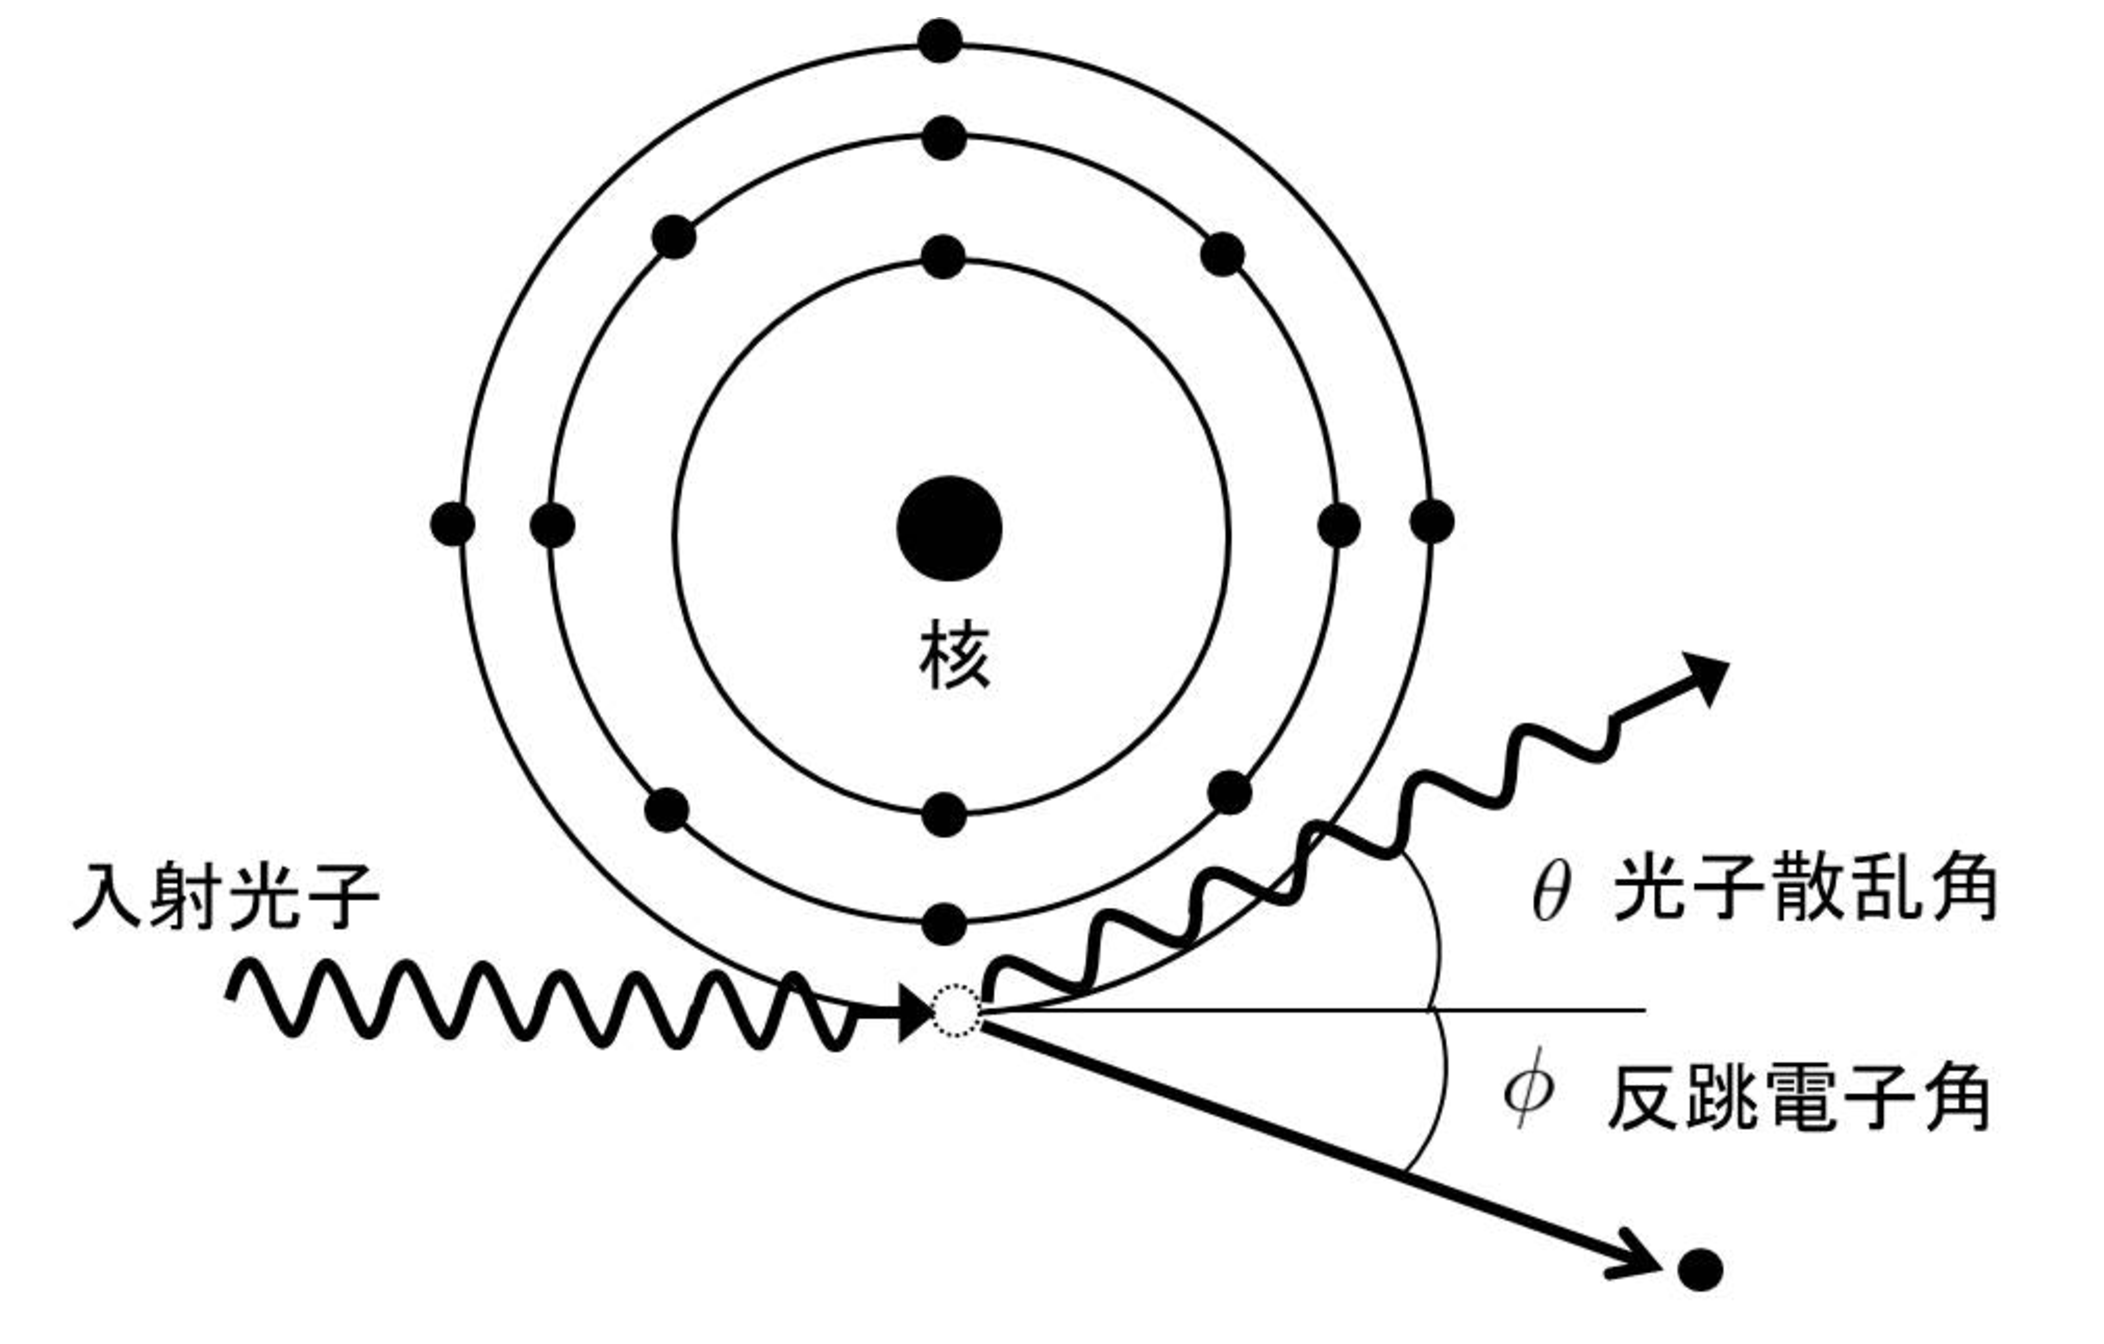
\includegraphics[width=10cm]{image/other/compton.eps}
 \end{center}
 \caption{コンプトン散乱}
 \label{fig:comp_geo}
\end{figure}

散乱光子のエネルギー$h\nu^{\prime}$はエネルギー保存則,運動量保存則より
\begin{align}
h\nu^{\prime}=\frac{h\nu}{1+\displaystyle\frac{h\nu}{m_oc^2}(1-\cos{\theta})} \label{eq:comp1}
\end{align}
と書くことができる。ここで$m_0c^2$は電子の静止質量エネルギー(0.511MeV)である。一方で反跳電子のエネルギー$E_r$は入射光子のエネルギーから,散乱線のエネルギーを差し引くだけなので,次式から容易に求めることができる。
\begin{align}
E_r=h\nu-h\nu^{\prime}=h\nu\left\{1-\frac{1}{1+\displaystyle\frac{h\nu}{m_0c^2}(1-\cos{\theta})}\right\} \label{eq:comp2}
\end{align}
\Eref{eq:comp2}より$\cos{\theta=1}$つまり$\theta=0^{\circ}$,すなわち散乱線が入射光子の入射方向と同じ方向に散乱されるとき$E_r=0$であり,エネルギーは反跳電子に伝達されず$h\nu^{\prime}=h\nu$となり,コンプトン散乱は起こらなかったことになる。一方で$\cos{\theta=-1}$つまり$\theta=180^{\circ}$,すなわち散乱線が入射光子の入射方向と反対方向に散乱されるとき$E_r$は最大となり
\begin{align}
E_{r\ \rm max}=h\nu\cdot\frac{1}{1+\displaystyle\frac{m_0c^2}{2h\nu}} \label{eq:comp_edge}
\end{align}
となる。このときの$E_{r\ \rm max}$とコンプトンエッジという。このとき,散乱線のエネルギーは最小となり\Eref{eq:comp1}より,
\begin{align}
h\nu^{\prime}_{\rm min}=\frac{h\nu}{1+\displaystyle\frac{2h\nu}{m_0c^2}} \label{eq:nyu_min}
\end{align}
となる。反跳電子のエネルギースペクトルは$E_r=0からE_{r\ \rm max}$まで分布し,連続スペクトルとなる。\\
\ \ 入射光子のエネルギーが比較的低いとき($h\nu\ll m_0c^2$),高いとき($h\nu\gg m_0c^2$)の散乱線の振る舞いを考える。まず入射光子のエネルギーが比較的低いときは,散乱線のエネルギーは\Eref{eq:comp1}より角度によらず$h\nu^{\prime}\fallingdotseq h\nu$で$E_r\fallingdotseq0$となり,これは入射光子が微小角だけ散乱され進行方向が変わるだけのトムソン散乱である。一方で入射光子のエネルギーが比較的高いときは$h\nu^{\prime}\fallingdotseq m_0c^2/(1-\cos{\theta})$となる。従って,$\theta=90^{\circ}$方向の散乱線のエネルギーは入射光子のエネルギーに関係なく0.51MeVとなり,$\theta=180^{\circ}$方向の散乱線のエネルギーはその半分の0.26MeVになる。\\
\ \ 散乱線の角度分布は角度$\theta$方向の微小立体角$d\Omega$に対する微分散乱断面積で表せる。それはクライン-仁科の式より以下で与えられる。
\begin{align}
\frac{\sigma_{\rm comp}}{d\Omega}=Z\cdot\frac{r_0^2}{2}(1+\cos^2{\theta})\cdot\left[\frac{1}{1+\alpha(1-\cos{\theta})}\right]^2\cdot\left[1+\frac{\alpha^2(1-\cos{\theta})^2}{(1+\cos^2{\theta})\{1+\alpha(1-\cos{\theta})\}}\right]
\end{align}
ここで$\alpha=h\nu/m_0c^2,r_0$は古典的電子半径であるこの分布は\Fref{fig:comp_sigma}に示すようになり,入射光子のエネルギーが高くなるにつれてコンプトン散乱の断面積は小さくなるが,前方散乱の割合が増大する。1個の原子あたりのコンプトン散乱の反応断面積$\sigma_{\rm comp}$は
\begin{align}
\sigma_{\rm comp}\propto\frac{Z}{E}\label{eq:sigma_comp}
\end{align}
と書ける。X線撮像に用いるエネルギー領域(40keV-140keV程度)ではコンプトン散乱は原子番号のみに依存する。

\begin{figure}[H]
 \begin{center}
 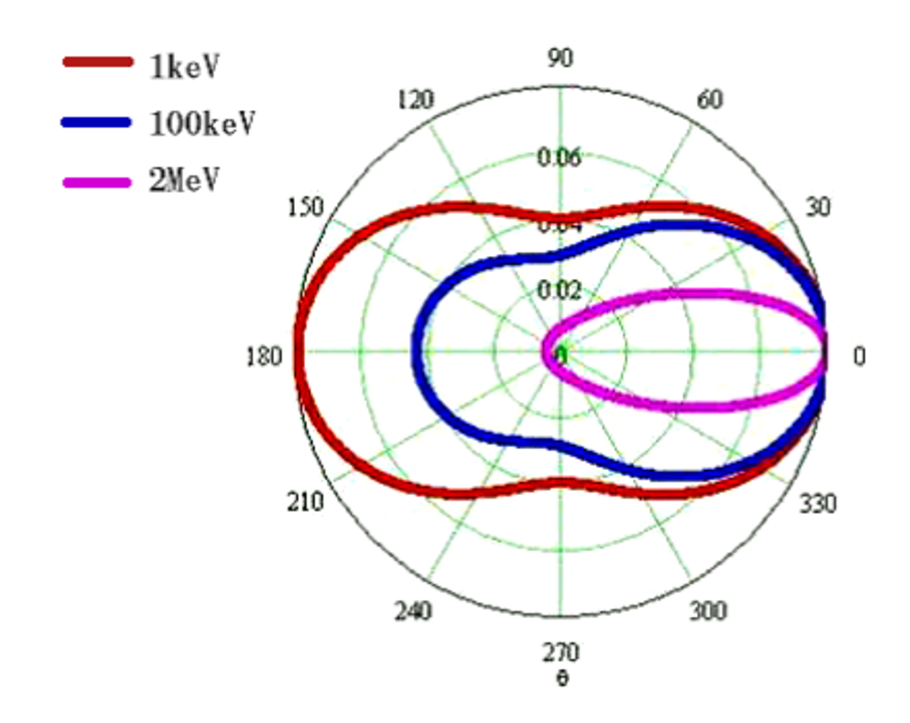
\includegraphics[width=10cm]{image/other/comp_cross.eps}
 \end{center}
 \caption{コンプトン散乱光子の角度分布\cite{nishidai}}
 \label{fig:comp_sigma}
\end{figure}

%
\if0
\subsection{電子$\cdot$陽電子対生成}
入射光子のエネルギーが電子の静止質量エネルギーの2倍すなわち,1.02MeVを越えると,コンプトン散乱は起こりにくくなるが電子対生成が起きるようになる。電子対生成とは1.02MeV以上の入射光子が原子の近くを通る際に,原子核のクーロン電場の中で光子が消滅し,代わって一対の電子と陽電子が生成される現象である(\Fref{fig:pair})。

\begin{figure}[H]
 \begin{center}
 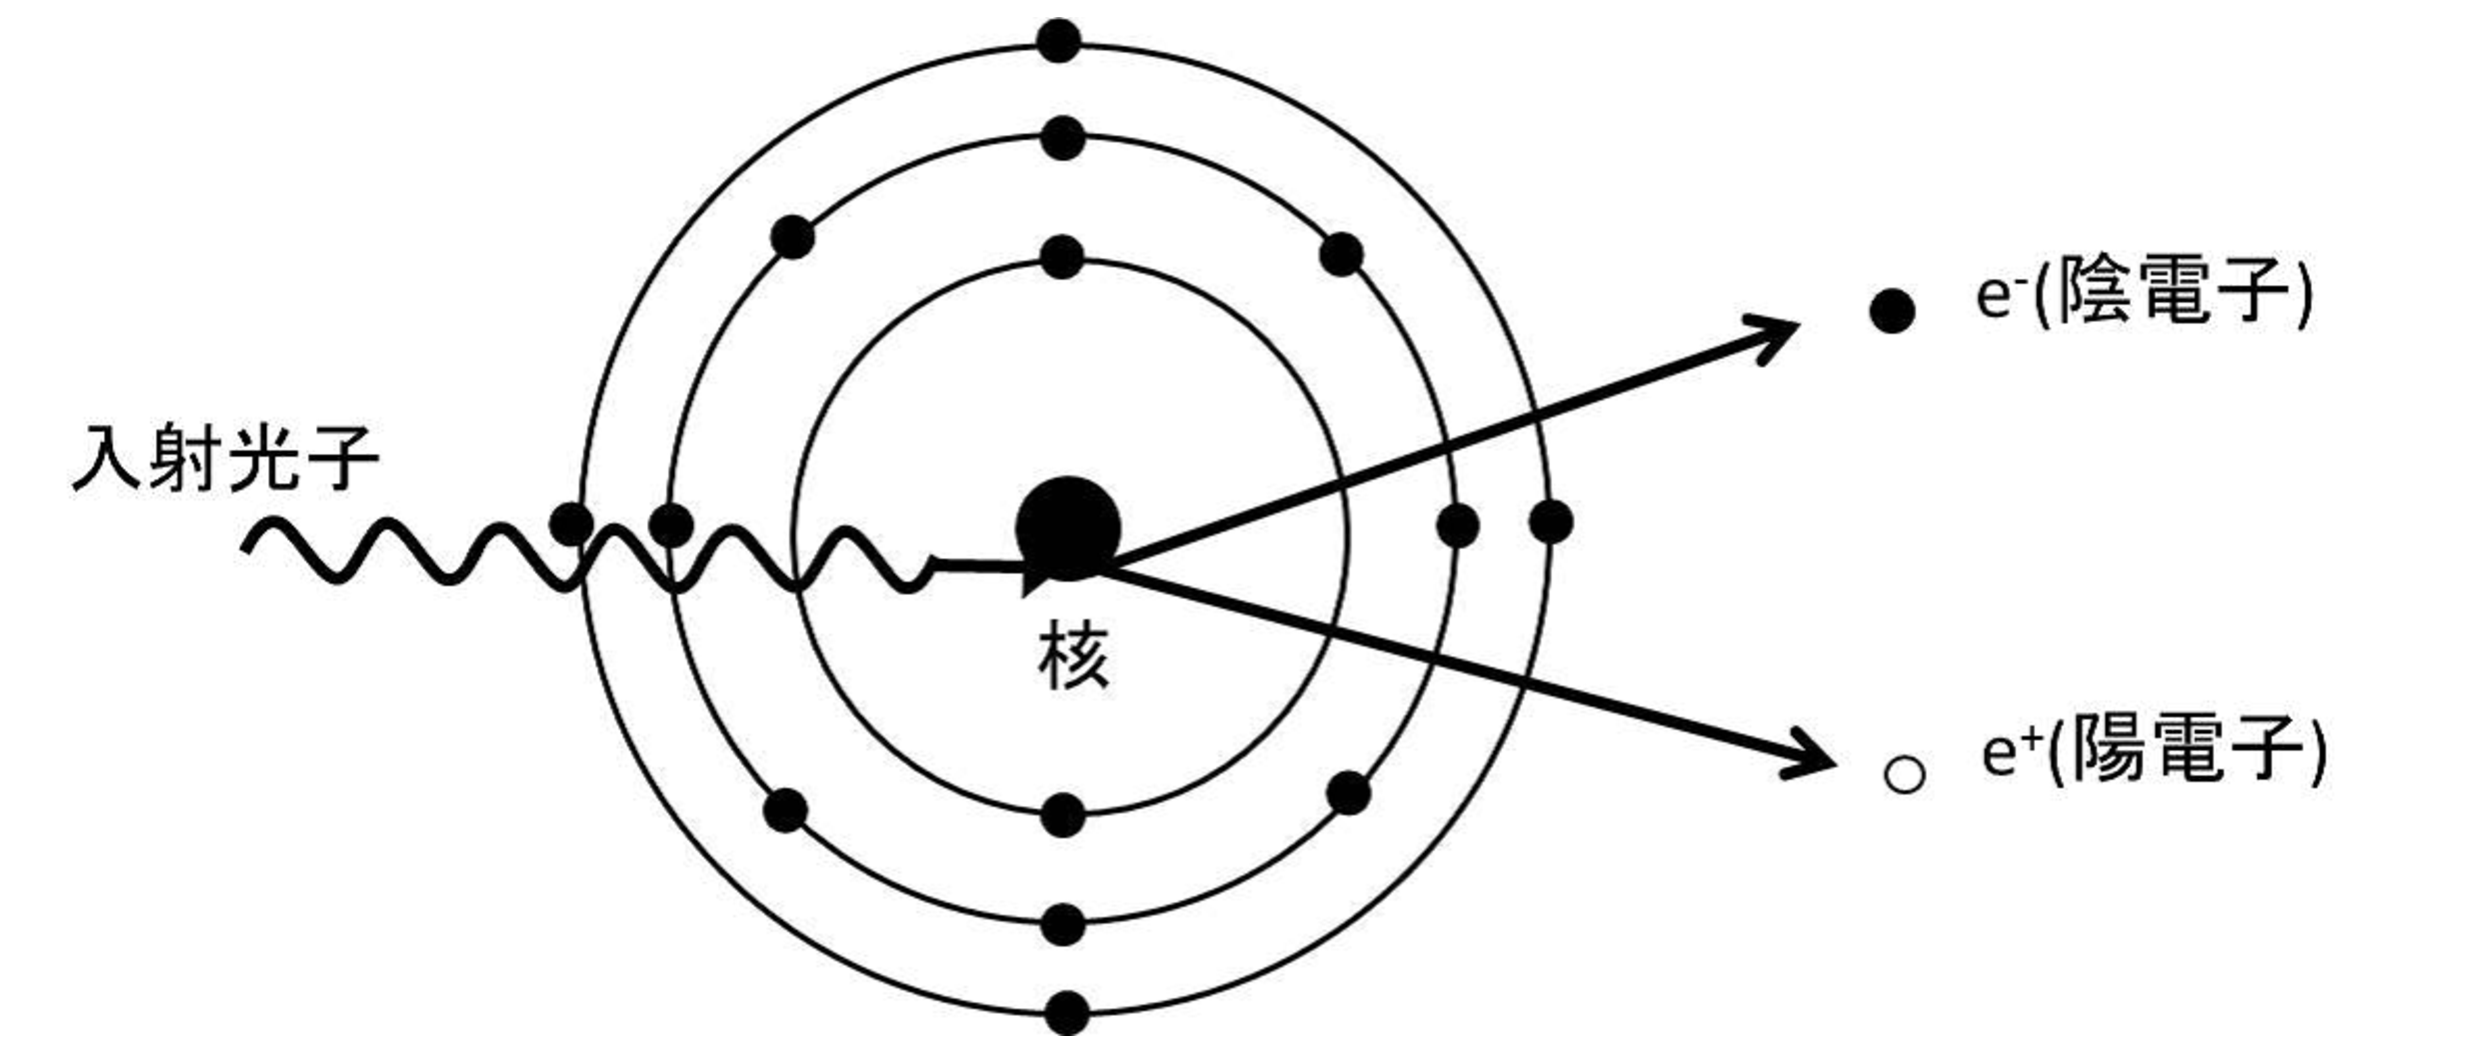
\includegraphics[width=10cm]{image/other/pair_create.eps}
 \end{center}
 \caption{電子対生成}
 \label{fig:pair}
\end{figure}


入射光子のエネルギーを$h\nu$,電子の静止質量エネルギーを$m_0c^2$,電子対生成によって生じた両電子の運動エネルギーを$E_+,E_-$とすると,エネルギーと質量の両保存則から次式が成り立つ。
\begin{align}
E_++E_-=h\nu-2m_0c^2 \label{eq:pair}
\end{align}
この式からわかるように,電子対生成では,入射光子のエネルギーの一部が両電子の質量静止エネルギーに転化し,残りがその運動エネルギーとなる。従って,電子対生成は入射光子のエネルギーが電子対の質量静止エネルギー1.02MeV($2m_0c^2$)より高くないと起こらない。また,電子対生成で生じた両電子の運動エネルギーは必ずしも等分配されず,$0からh\nu-2m_0c^2$まで広範囲にわたって分布する。1原子あたりの電子対生成の反応断面積$\sigma_{\rm pair}$は
\begin{align}
\sigma_{\rm pair}=Z^2(E-1.02) \label{eq:sigma_pair}
\end{align}
で表される。この式からわかるように,電子対生成は入射光子のエネルギーが高く,物質の原子番号が高いほど起こりやすい。

%
\fi

\section{X線の減弱\label{sec:atten}}

\begin{figure}[H]
 \begin{center}
 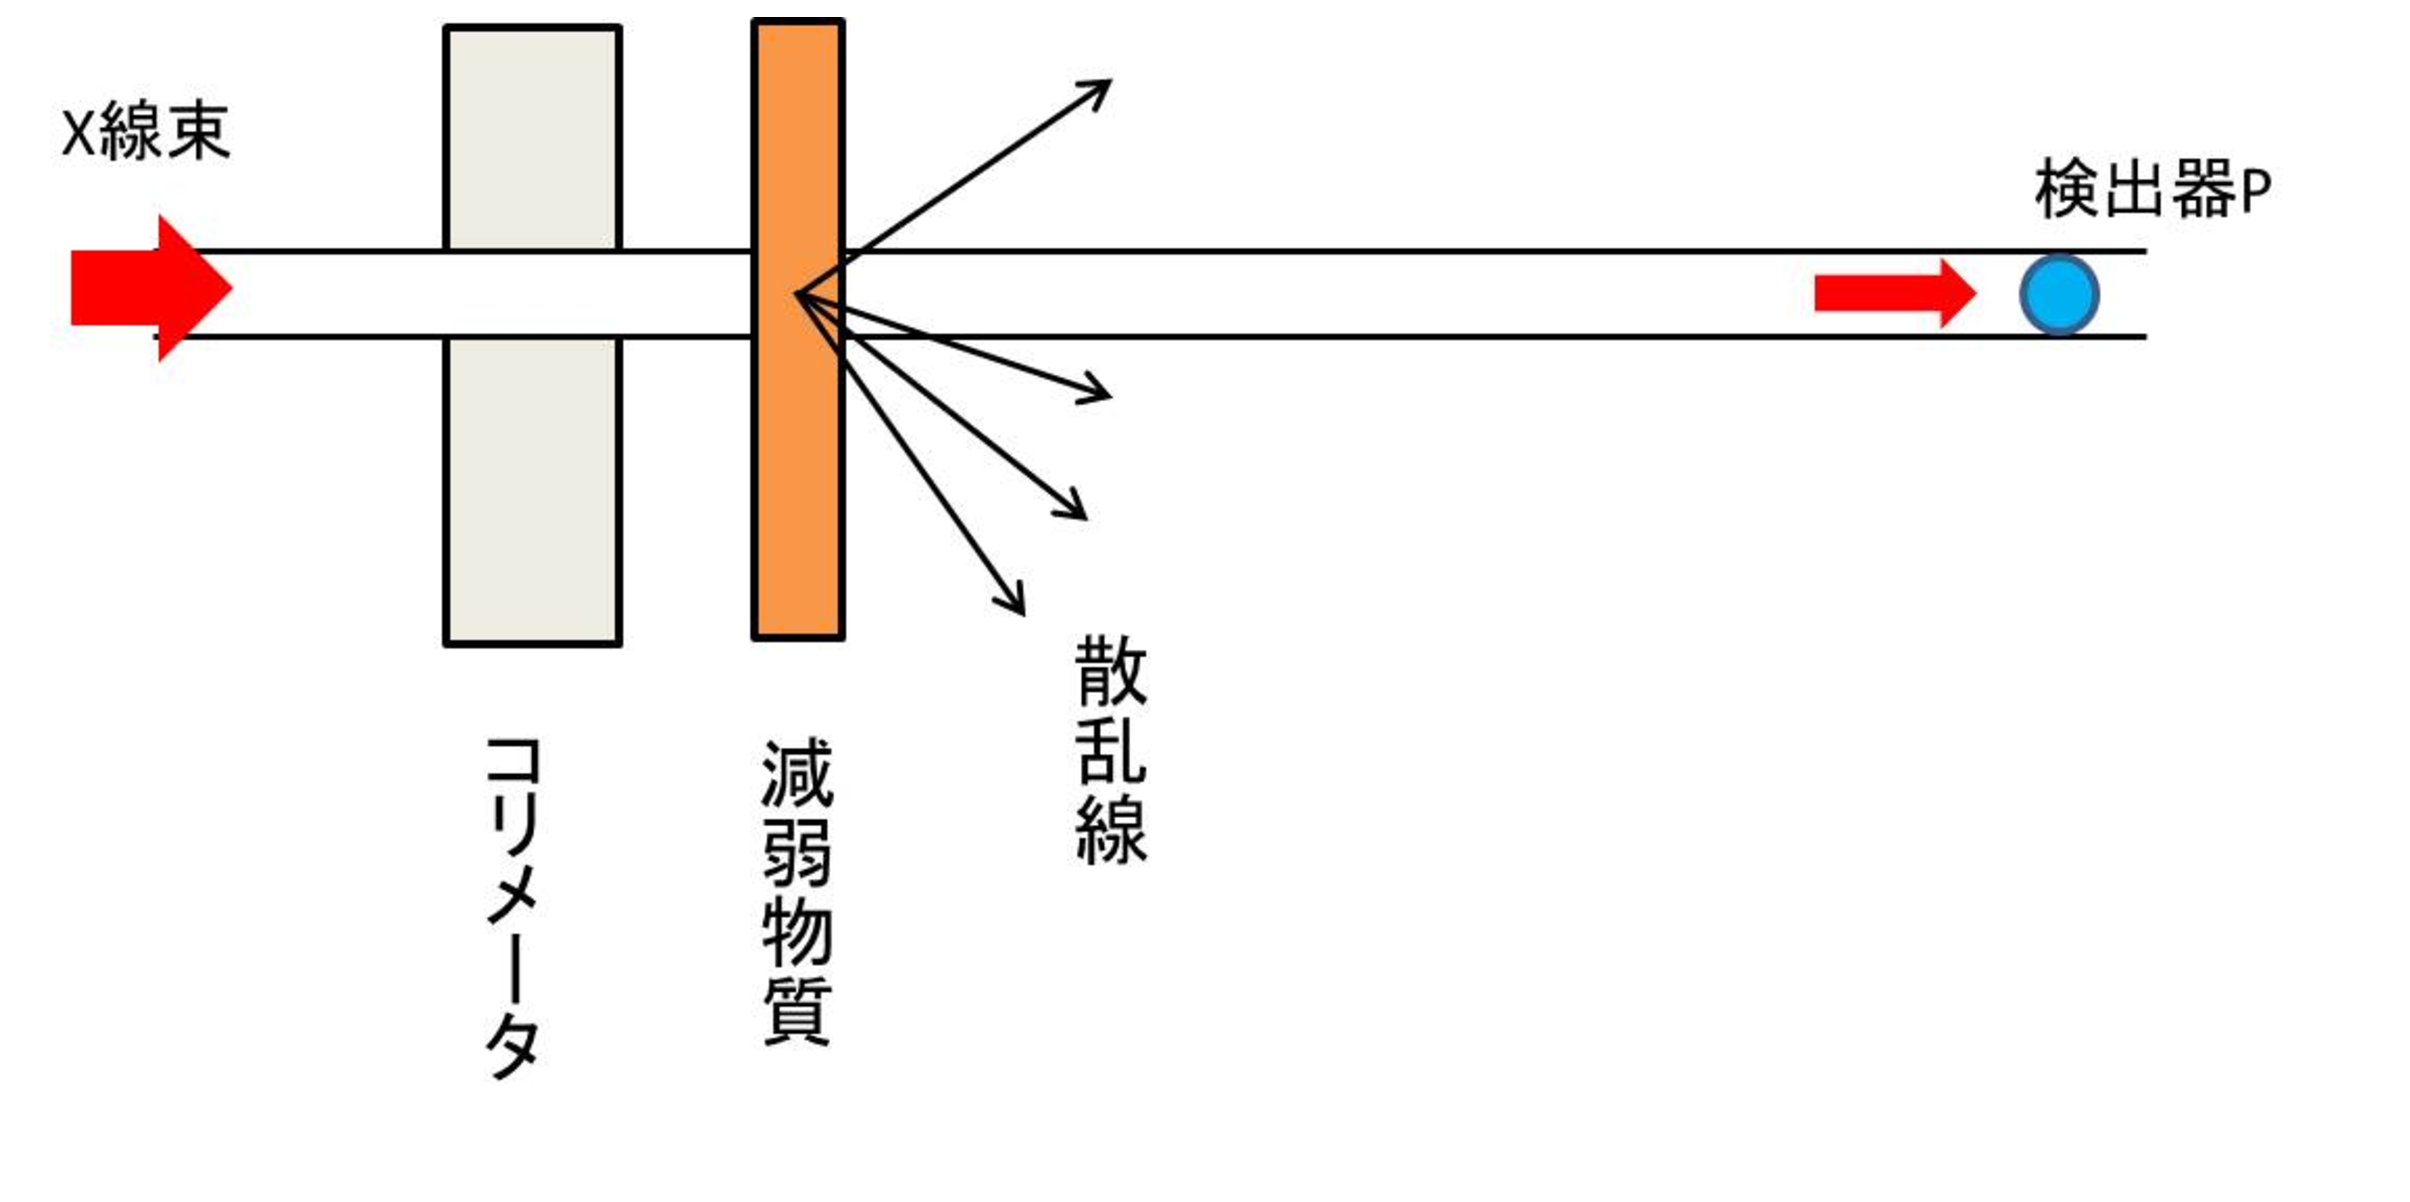
\includegraphics[width=10cm]{image/other/trans.eps}
 \end{center}
 \vspace{-1cm}
 \caption{X線束の物質による減弱測定}
 \label{fig:trans}
\end{figure}

\Fref{fig:trans}のような透過実験を想定し,この図で単一エネルギーのX線束(単色X線)あるいは$\gamma$線の物質中での減弱について考える。物質と全く相互作用を起こさず,X線束上の検出器Pに到達する透過光子数を求める。この場合,一度でも物質と相互作用をした散乱線はその進行方向が変わり,検出器Pに到達することができない。検出器Pに到達する透過光子数$I$は入射光子数と$I_0$,物質の厚さを$x$として
\begin{align}
I=I_0e^{-\mu x} \label{eq:atten}
\end{align}
と表せる。ここで$\mu$は線源弱係数であり単位は[1/cm]である。これは物質厚さ$x$を厚くすると指数関数的に減衰していく。\\
\ \ 本来,物質のある点において,ある光子が相互作用を起こすがどうかは全くの確率現象であり,その確率はポアソン分布に従うものである。すなわち\Eref{eq:atten}の$e^{-\mu x}$は光子が相互作用を起こさずに物質中を通過する確率を巨視(マクロ)的に表しており,その確率は主に光電吸収,コンプトン散乱,電子対生成の微視(ミクロ)的な相互作用による確率の積である。すなわち,
物質構成原子の1個あたりの全断面積$\sigma$
\begin{align}
\sigma=\sigma_{\rm photo}+\sigma_{\rm comp}+\sigma_{\rm pair} \label{eq:sigma_all}
\end{align}
に比例した値になる。各断面積は,
\begin{align}
\begin{cases}
\sigma_{\rm photo}\propto Z^{4-5}/E^{3.5}\\
\sigma_{\rm comp}\propto Z/E\\
\sigma_{\rm pair}\propto Z^2(E-1.02)
\end{cases}
\end{align}
である。したがって原子1個あたりの全断面積$\sigma$は原子番号$Z$と入射エネルギー$E$の複雑な関数となる。物質の単位体積あたりの原子数を$n$とすると,線源弱係数$\mu$は
\begin{align}
\mu&=n\sigma \\
&=n\sigma_{\rm photo}+n\sigma_{\rm comp}+n\sigma_{\rm pair}\\
&=\mu_{\rm photo}+\mu_{\rm comp}+\mu_{\rm pair}
\end{align}
となり,線減弱係数はそれぞれの相互作用における線減弱係数の和として表すことができる。\\
\ \ 線源弱係数$\mu$は同じ物質であってもその密度に依存して変化するために,一般に線源弱係数$\mu[\rm cm^{-1}]$を物質の密度$\rho[\rm g/cm^{3}]$で割った値が用いられる。これを質量減弱係数といい$\mu_m[\rm cm^2/g]$で表す。アボガドロ数を$N_A$,原子量を$A$とすると,1gあたりの原子数$n/\rho=N_A/A$なので%アボガドロ数個の原子の個数分の重さが原子量
\begin{align}
\mu_m=\frac{\mu}{\rho}=\frac{n\sigma}{\rho}=\frac{N_A}{A}\sigma \label{eq:mass_atten}
\end{align}
となる。この式から$\mu_m$は物質の密度には関係せず,原子番号と入射光子のエネルギーのみに依存することがわかる。線源弱係数は同じ物質であってもその密度によって依存する,また物質が異なっても密度によっては同一になる場合があるが,質量減弱係数は物質に固有な値なので,線源弱係数より便利である(\Fref{fig:atten})。

\begin{figure}[H]
 \begin{minipage}{0.52\hsize}
  \begin{center}
   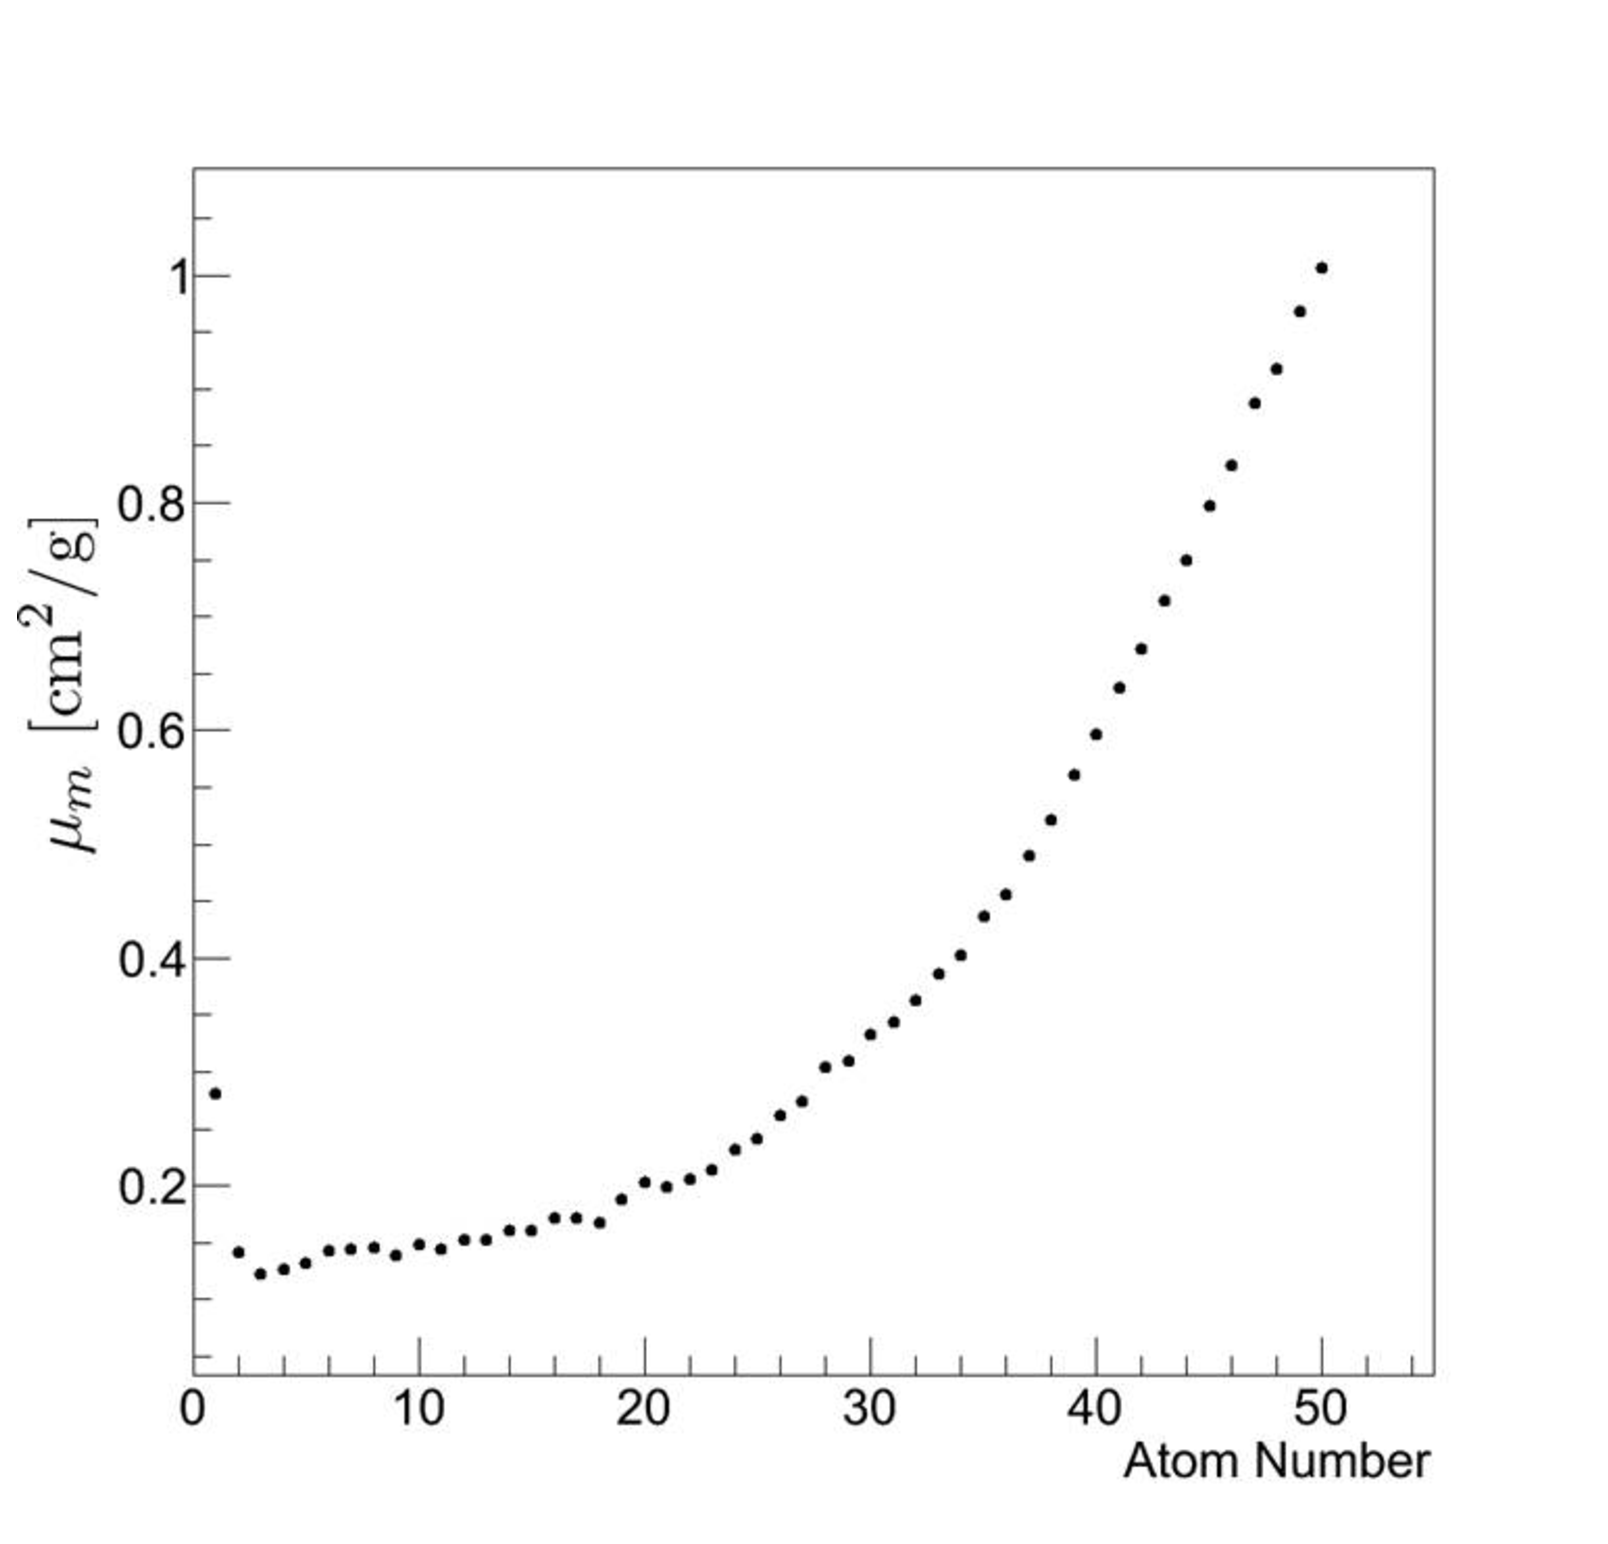
\includegraphics[width=7cm]{image/other/mass_atten.eps}
  \end{center}
   \vspace{-0.5cm}
    \caption*{質量減弱係数の原子番号依存性}
 \end{minipage}
 \begin{minipage}{0.52\hsize}
  \begin{center}
   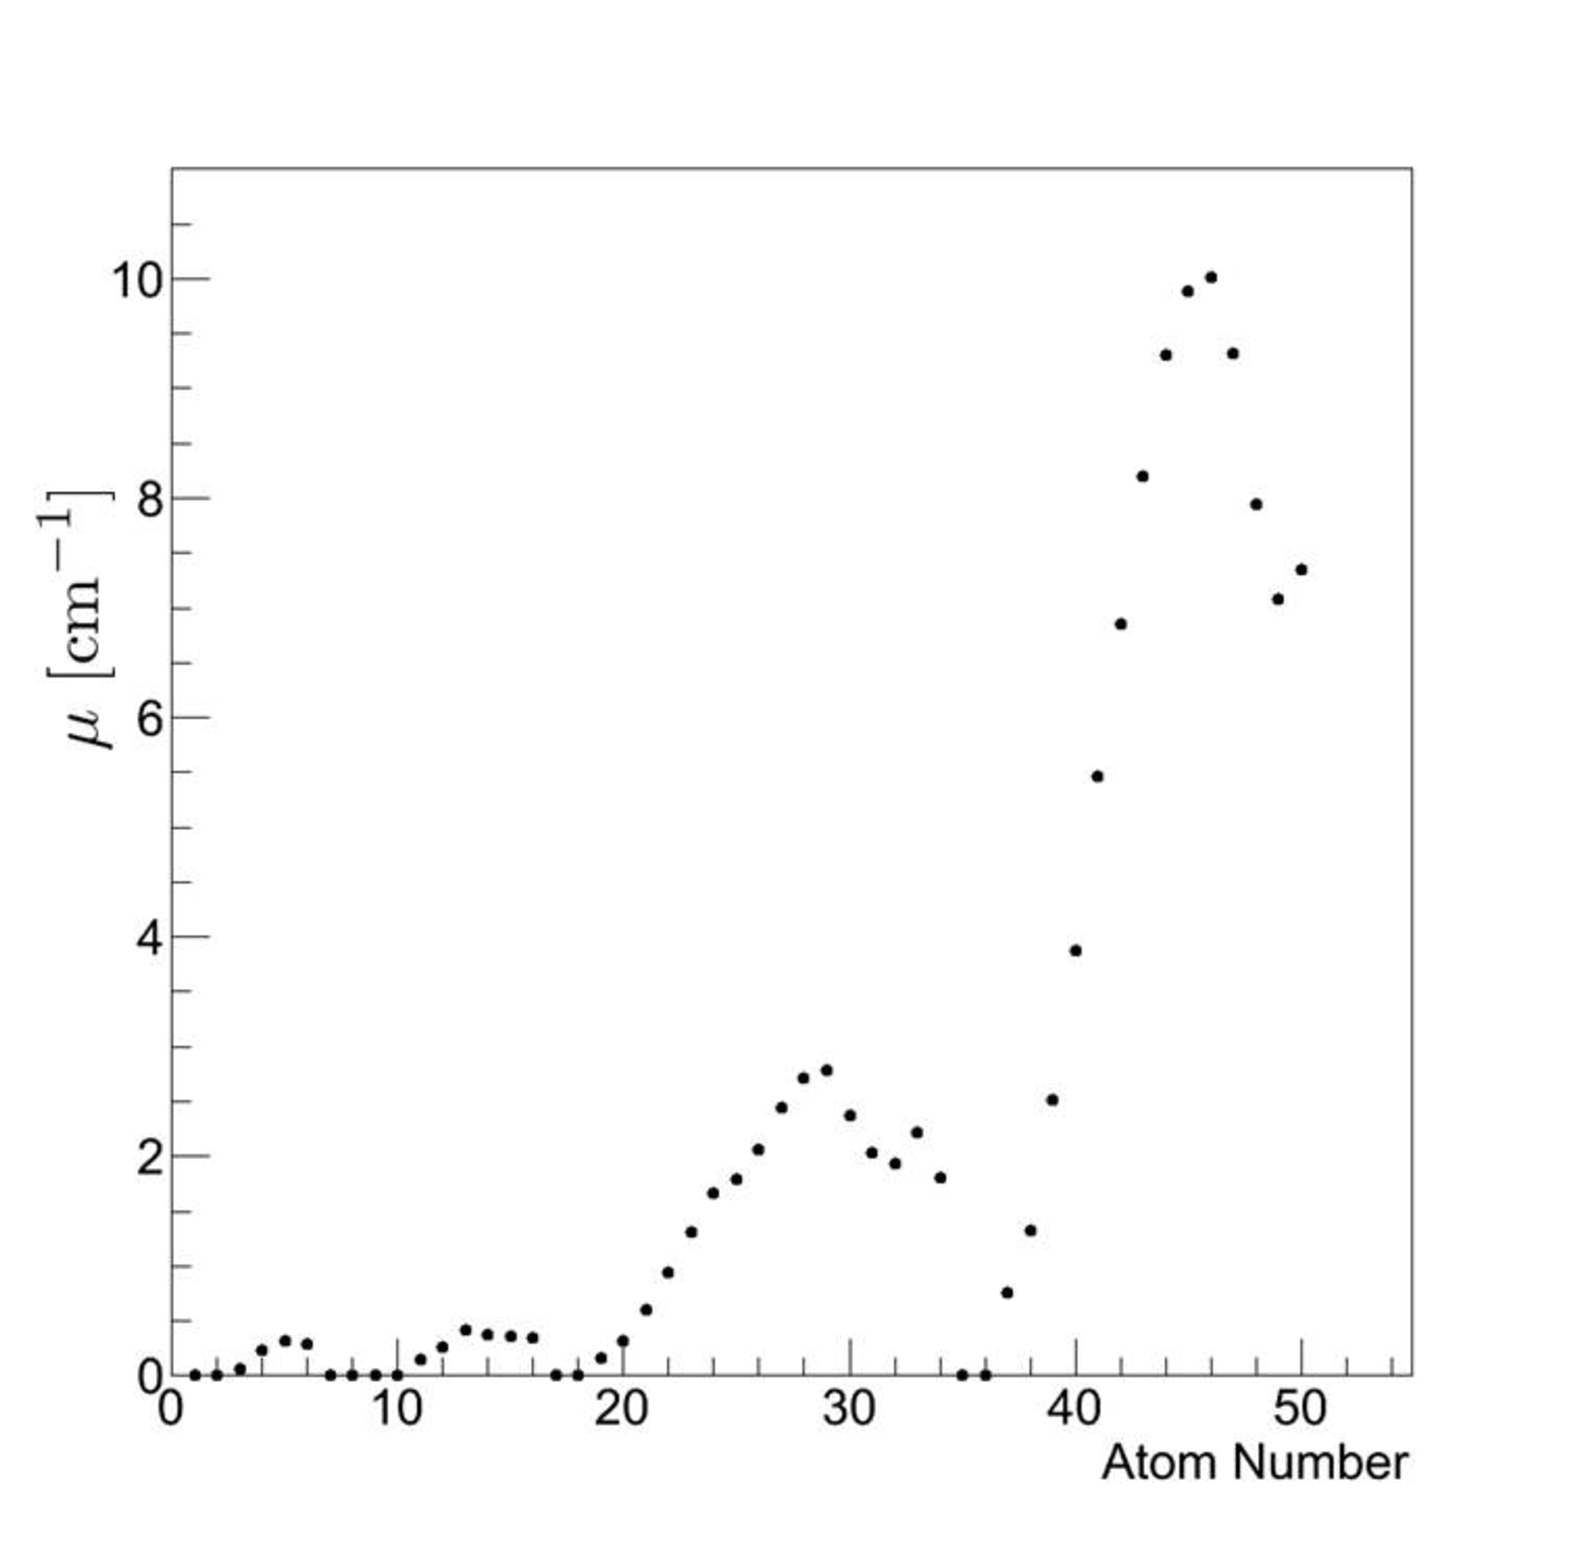
\includegraphics[width=7cm]{image/other/linear_atten.eps}
  \end{center}
     \vspace{-0.5cm}
   \caption*{線減弱係数の原子番号依存性}
 \end{minipage}
 \begin{center}
  \vspace{-1zh}
  \caption{質量減弱係数の原子番号依存性と線源弱係数の原子番号依存性(@122keV)\newline 質量減弱係数はエネルギーが一定であれば物質によって異なる値を取るが,線源弱係数は物質が異なっても密度によっては同一になる場合がある}
  \label{fig:atten}
  \end{center}
\end{figure}



\ \ \Fref{fig:mass_atten}は一例として,NaI(Tl)の線減弱係数$\mu$とそれを構成する光電吸収,コンプトン散乱,電子対生成のそれぞれの線減弱係数が入射光子のエネルギーによってどのように変化するかを示したものであり,\Fref{fig:mu_dist}は入射光子エネルギーと光電吸収,コンプトン散乱,電子対生成の各相互作用の優勢領域を示したものである。

\begin{figure}[H]
 \begin{center}
 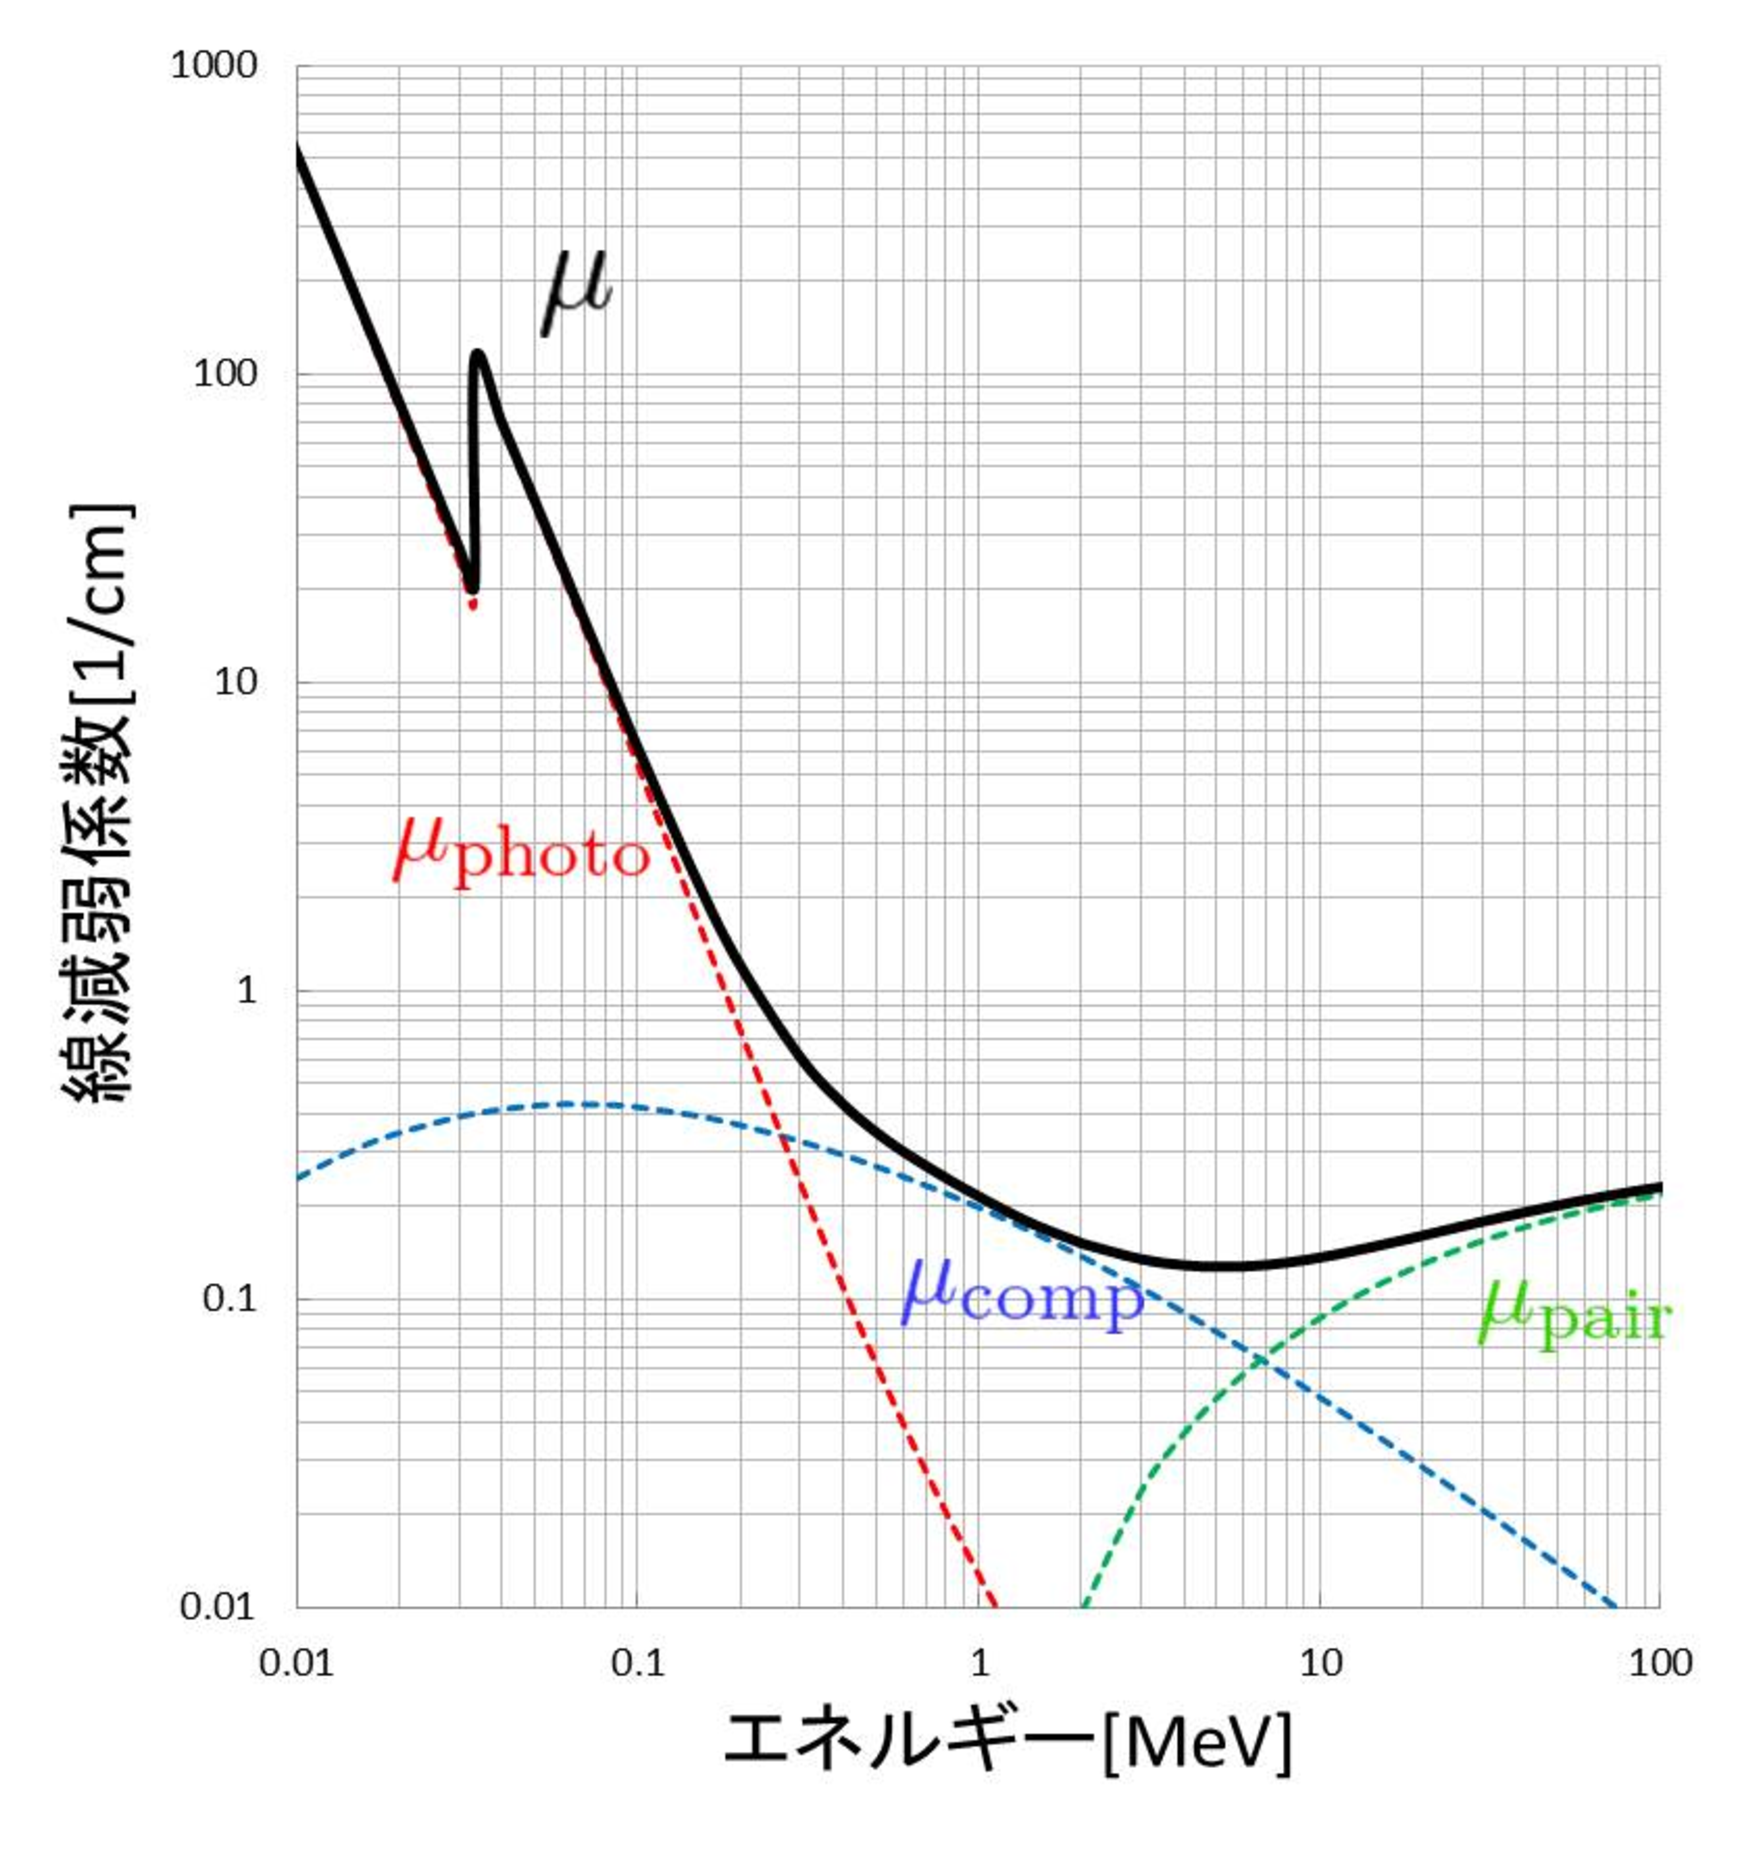
\includegraphics[width=8cm]{image/other/NaI_mu.eps}
 \end{center}
 \caption{NaI(Tl)の線減弱係数とその成分[NIST\cite{nist}より作成]}
 \label{fig:mass_atten}
\end{figure}

\begin{figure}[H]
 \begin{center}
 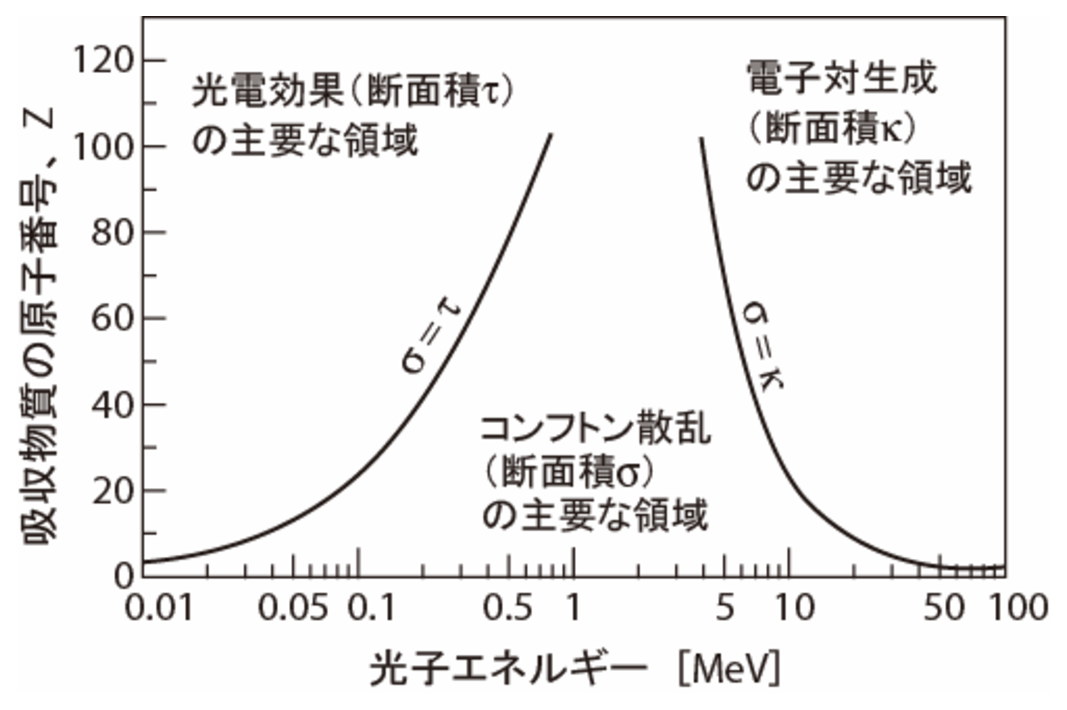
\includegraphics[width=10cm]{image/other/mu_dist.eps}
 \end{center}
 \caption{電磁放射線と物質との相互作用の優勢領域\cite{QA}}
 \label{fig:mu_dist}
\end{figure}











